\documentclass[a4paper, 10pt,onecolumn]{scrartcl}
\usepackage[ngerman]{babel}
\usepackage[T1]{fontenc}
\usepackage[utf8]{inputenc}
\usepackage{multirow}
\usepackage{natbib}
\usepackage{graphicx}
\usepackage{amsmath, amssymb}
\usepackage{graphicx}
\usepackage{grffile} %einfacheres einbinden von Dateipfaden


\title{Schlechte Bilder\thanks{Danke an John Wigg}} 
\author{Ich} %auch nach \begindocument möglich
\date{\today}
\setlength{\parindent}{0pt}

\begin{document}
\tableofcontents
\listoffigures
\maketitle

\section{Bilder in \LaTeX}
Wenn Bilder eingebunden werden, stehen sie standardmäßig auf der Grundlinie: 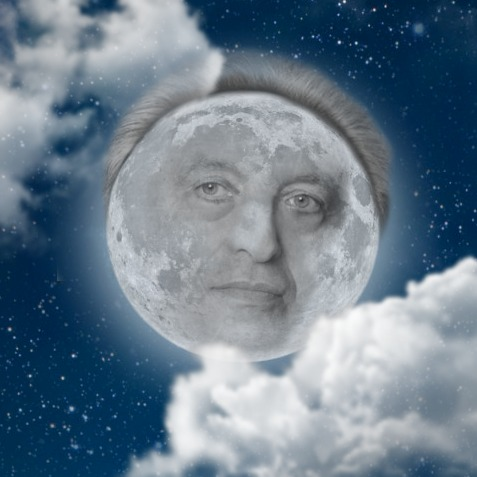
\includegraphics[width=11pt]{lotze.jpg}.
Dies kann nützlich sein, wenn man ein bestimmtes Symbol nur als Bild vorliegen hat. Im Normalfall möchte man das Bild jedoch meist zentrieren. Wenn das Bild zu groß ist, muss es skaliert werden:

\begin{figure}[ht!]
	\centering
	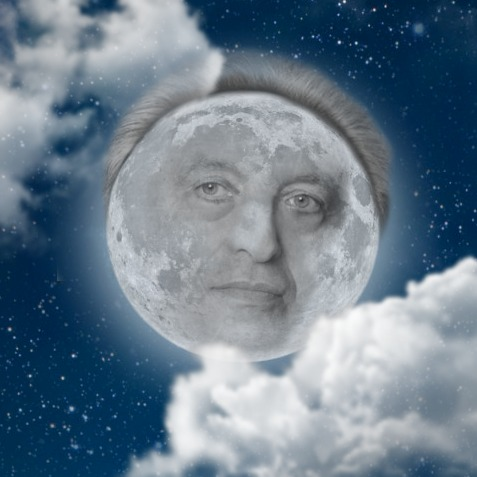
\includegraphics[scale=0.5]{lotze.jpg}
	\caption{Nicht die Sombrero-Galaxie}
	\label{Lotze}
\end{figure}
\newpage

\subsection{Skalieren und Beschneiden}
Durch die Angabe von Höhe und Breite kann \eqref{Lotze} verzerrt werden.

\begin{center}
	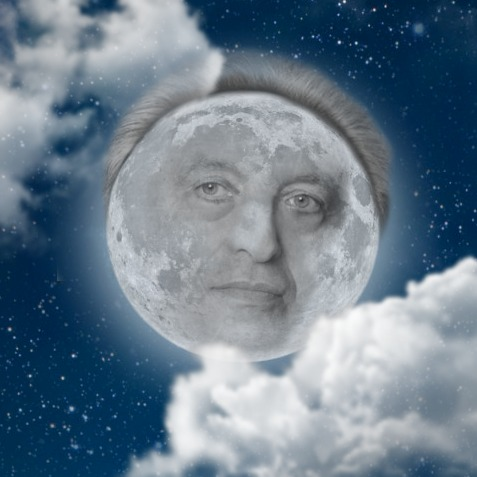
\includegraphics[width=10cm, height= 5cm]{lotze.jpg}
\end{center}

Das Bild kann auch zugeschnitten werden:

\begin{center}
	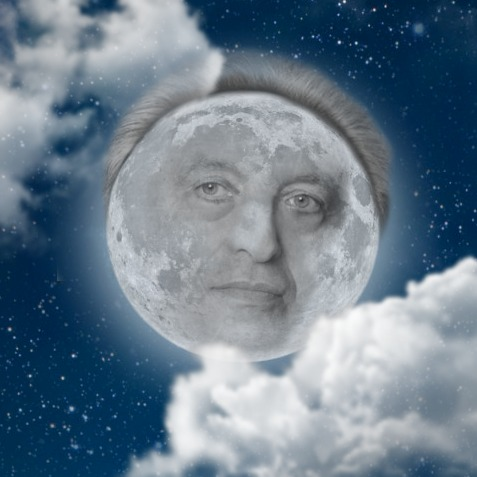
\includegraphics[clip, trim=7cm 7cm 5cm 6cm]{lotze.jpg}
	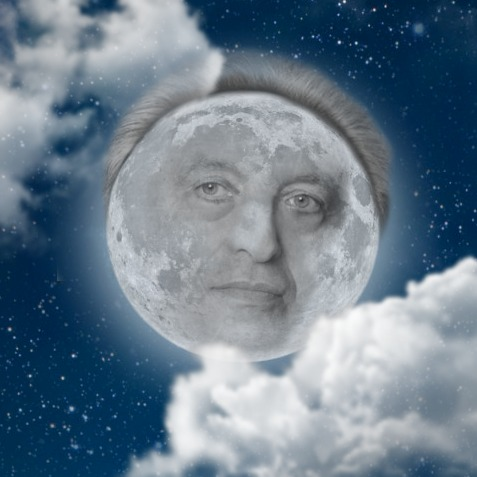
\includegraphics[clip, trim=7cm 7.5cm 6cm 7.5cm]{lotze.jpg}
\end{center}
\newpage
\subsection{PDFs als Bilder}
Dies ist mein erstes \LaTeX-Dokument, eingebunden als Bild:
\begin{center}
	
\includegraphics[scale=0.25, page=2]{hellooworld.pdf}
\end{center}
Hier nochmal mit einem Rahmen:
\begin{center}
	\fbox{
\includegraphics[scale=0.25,page=2]{hellooworld.pdf}}
\end{center}


	

\end{document}